\documentclass[tikz, border=10pt]{standalone}
\usepackage{xcolor}
\usetikzlibrary{
    positioning,     % For relative positioning of nodes (e.g., right=of)
    arrows.meta,     % For modern arrow tips like Stealth
    shadings,        % For creating gradient fills
    shapes.geometric % For node shapes like rectangle
}

% --- Custom Color Definitions ---
% Define a light blue-gray for the page background to match the image
\definecolor{bgcolor}{RGB}{240,243,248}
% Define a dark blue for node borders
\definecolor{bordercolor}{RGB}{30,32,82}
% Define gradient colors for 'Conv' and 'Split' nodes (light blue to light purple)
\definecolor{convleft}{RGB}{208,222,255}
\definecolor{convright}{RGB}{230,220,255}
% Define gradient colors for 'Bottleneck' nodes (yellowish to pink)
\definecolor{bottleleft}{RGB}{255,220,170}
\definecolor{bottleright}{RGB}{255,210,230}
% Define gradient colors for 'Concat' node (light blue to red)
\definecolor{concatleft}{RGB}{190,220,255}
\definecolor{concatright}{RGB}{255,100,120}

% --- Page Style ---
% Set the background color for the entire document
\pagecolor{bgcolor}

% --- Custom Shading Definitions ---
% These create the horizontal color gradients used to fill the nodes.
\pgfdeclarehorizontalshading{convshading}{100bp}{
  color(0bp)=(convleft);
  color(100bp)=(convright)
}
\pgfdeclarehorizontalshading{bottleshading}{100bp}{
  color(0bp)=(bottleleft);
  color(100bp)=(bottleright)
}
\pgfdeclarehorizontalshading{concatshading}{100bp}{
  color(0bp)=(concatleft);
  color(100bp)=(concatright)
}

\begin{document}
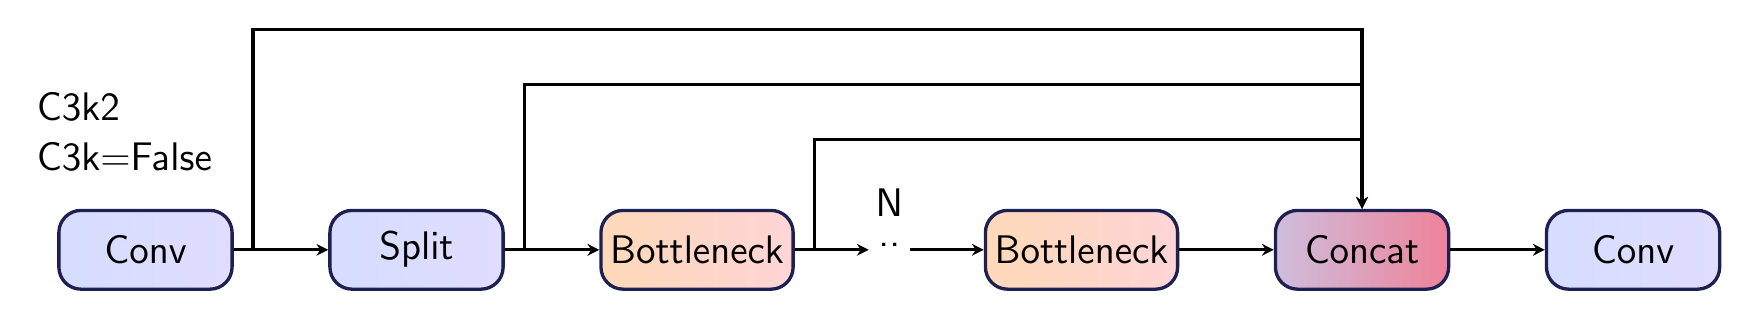
\begin{tikzpicture}[
    % Set default font to sans-serif for the entire picture
    font=\sffamily,
    % Define a general style for the rectangular blocks
    >={Stealth[length=1.5mm, width=1.5mm]},
    block/.style={
        rectangle, 
        rounded corners=8pt, 
        draw=bordercolor, 
        very thick, 
        text=black, 
        minimum height=1cm, 
        minimum width=2.2cm, 
        font=\sffamily\Large, 
        align=center
    },
    % Define a style for the arrows for consistency
    arrow/.style={
        % -{{Stealth[length=3mm, width=3mm]}}, % Arrow tip style
        very thick,
        draw=black
    }    
]

% --- Node Placement ---
% Nodes are placed sequentially from left to right using the 'positioning' library.
\node[block, shading=convshading] (conv1) {Conv};

\node[block, shading=convshading, right=1.2cm of conv1] (split) {Split};

\node[block, shading=bottleshading, right=1.2cm of split] (bottle1) {Bottleneck};

% This second bottleneck is placed further away to leave space for the 'N..' text.
\node[block, shading=bottleshading, right=2.4cm of bottle1] (bottle2) {Bottleneck};

\node[block, shading=concatshading, right=1.2cm of bottle2] (concat) {Concat};

\node[block, shading=convshading, right=1.2cm of concat] (conv2) {Conv};

% --- Intermediate Labels (N..) ---
% A 'path' is used to place the 'N..' text midway between the two bottleneck nodes
% without drawing anything.
\path (bottle1.east) -- (bottle2.west) 
    node[midway, font=\sffamily\Large] (dots) {\raisebox{0.5ex}{..}}
    node[above=0.1cm of dots, font=\sffamily\Large] {N};

% --- Text Labels (C3k) ---
% Define a coordinate for the start of the first skip connection's vertical line.
\coordinate (c1_start) at ([xshift=7pt]conv1.east);
% Place the labels relative to this starting point for precise alignment.
\node[align=left, font=\sffamily\Large, anchor=east] at ([xshift=-4mm, yshift=1.5cm]c1_start) {C3k2 \\ C3k=False};

% --- Arrow Drawing ---
% Main sequential path connecting the blocks.
\draw[->, arrow] (conv1)  --  (split);
\draw[->, arrow] (split) -- (bottle1);
% The arrow from bottle1 goes to the 'dots' node, and from there to bottle2.
\draw[->, arrow] (bottle1) -- (dots);
\draw[->, arrow] (dots) -- (bottle2);
\draw[->, arrow] (bottle2) -- (concat);
\draw[->, arrow] (concat) -- (conv2);

% --- Skip Connections ---
% These connections are drawn using the |- and -| path operators for right-angled lines.
% Define start points slightly to the right of the blocks for the vertical lines.

\coordinate (s1_start) at ([xshift=7pt]split.east);
\coordinate (b1_start) at ([xshift=7pt]bottle1.east);

% Path from 'Conv' to 'Concat' (topmost path)
\draw[->, arrow ] (c1_start) |- ++(1, 2.8cm) -| (concat.north);

% Path from 'Split' to 'Concat' (middle path)
\draw[->, arrow] (s1_start) |- ++(1, 2.1cm) -| (concat.north);

% Path from 'Bottleneck' to 'Concat' (bottom path)
\draw[->, arrow] (b1_start) |- ++(1, 1.4cm) -| (concat.north);

\end{tikzpicture}
\end{document}